\documentclass{article}\usepackage[]{graphicx}\usepackage[]{color}
%% maxwidth is the original width if it is less than linewidth
%% otherwise use linewidth (to make sure the graphics do not exceed the margin)
\makeatletter
\def\maxwidth{ %
  \ifdim\Gin@nat@width>\linewidth
    \linewidth
  \else
    \Gin@nat@width
  \fi
}
\makeatother

\definecolor{fgcolor}{rgb}{0.345, 0.345, 0.345}
\newcommand{\hlnum}[1]{\textcolor[rgb]{0.686,0.059,0.569}{#1}}%
\newcommand{\hlstr}[1]{\textcolor[rgb]{0.192,0.494,0.8}{#1}}%
\newcommand{\hlcom}[1]{\textcolor[rgb]{0.678,0.584,0.686}{\textit{#1}}}%
\newcommand{\hlopt}[1]{\textcolor[rgb]{0,0,0}{#1}}%
\newcommand{\hlstd}[1]{\textcolor[rgb]{0.345,0.345,0.345}{#1}}%
\newcommand{\hlkwa}[1]{\textcolor[rgb]{0.161,0.373,0.58}{\textbf{#1}}}%
\newcommand{\hlkwb}[1]{\textcolor[rgb]{0.69,0.353,0.396}{#1}}%
\newcommand{\hlkwc}[1]{\textcolor[rgb]{0.333,0.667,0.333}{#1}}%
\newcommand{\hlkwd}[1]{\textcolor[rgb]{0.737,0.353,0.396}{\textbf{#1}}}%

\usepackage{framed}
\makeatletter
\newenvironment{kframe}{%
 \def\at@end@of@kframe{}%
 \ifinner\ifhmode%
  \def\at@end@of@kframe{\end{minipage}}%
  \begin{minipage}{\columnwidth}%
 \fi\fi%
 \def\FrameCommand##1{\hskip\@totalleftmargin \hskip-\fboxsep
 \colorbox{shadecolor}{##1}\hskip-\fboxsep
     % There is no \\@totalrightmargin, so:
     \hskip-\linewidth \hskip-\@totalleftmargin \hskip\columnwidth}%
 \MakeFramed {\advance\hsize-\width
   \@totalleftmargin\z@ \linewidth\hsize
   \@setminipage}}%
 {\par\unskip\endMakeFramed%
 \at@end@of@kframe}
\makeatother

\definecolor{shadecolor}{rgb}{.97, .97, .97}
\definecolor{messagecolor}{rgb}{0, 0, 0}
\definecolor{warningcolor}{rgb}{1, 0, 1}
\definecolor{errorcolor}{rgb}{1, 0, 0}
\newenvironment{knitrout}{}{} % an empty environment to be redefined in TeX

\usepackage{alltt}
\IfFileExists{upquote.sty}{\usepackage{upquote}}{}
\begin{document}

\begin{knitrout}
\definecolor{shadecolor}{rgb}{0.969, 0.969, 0.969}\color{fgcolor}\begin{kframe}
\begin{alltt}
\hlcom{# GUIA 21 }

\hlcom{#Se digitan los datos del grupo de control }
\hlstd{IMC_Control} \hlkwb{<-} \hlkwd{c}\hlstd{(}\hlnum{23.6}\hlstd{,} \hlnum{22.7}\hlstd{,} \hlnum{21.2}\hlstd{,} \hlnum{21.7}\hlstd{,} \hlnum{20.7}\hlstd{,} \hlnum{22.0}\hlstd{,} \hlnum{21.8}\hlstd{,} \hlnum{24.2}\hlstd{,} \hlnum{20.1}\hlstd{,} \hlnum{21.3}\hlstd{,}
                 \hlnum{20.5}\hlstd{,} \hlnum{21.1}\hlstd{,} \hlnum{21.4}\hlstd{,} \hlnum{22.2}\hlstd{,} \hlnum{22.6}\hlstd{,} \hlnum{20.4}\hlstd{,} \hlnum{23.3}\hlstd{,} \hlnum{24.8}\hlstd{)}
\hlkwd{par}\hlstd{(}\hlkwc{mfrow}\hlstd{=}\hlkwd{c}\hlstd{(}\hlnum{1}\hlstd{,}\hlnum{2}\hlstd{))}
\hlkwd{hist}\hlstd{(IMC_Control,}\hlkwc{main}\hlstd{=}\hlstr{"A"}\hlstd{,}\hlkwc{xlab}\hlstd{=}\hlstr{"IMC (kg/m2)"}\hlstd{,}\hlkwc{ylab}\hlstd{=}\hlstr{"Frecuencia"}\hlstd{)}
\hlkwd{boxplot}\hlstd{(IMC_Control,}\hlkwc{main}\hlstd{=}\hlstr{"B"}\hlstd{,} \hlkwc{lab}\hlstd{=}\hlstr{"IMC (kg/m2)"}\hlstd{,}\hlkwc{ylim}\hlstd{=}\hlkwd{c}\hlstd{(}\hlnum{20}\hlstd{,}\hlnum{25}\hlstd{))}
\end{alltt}
\end{kframe}
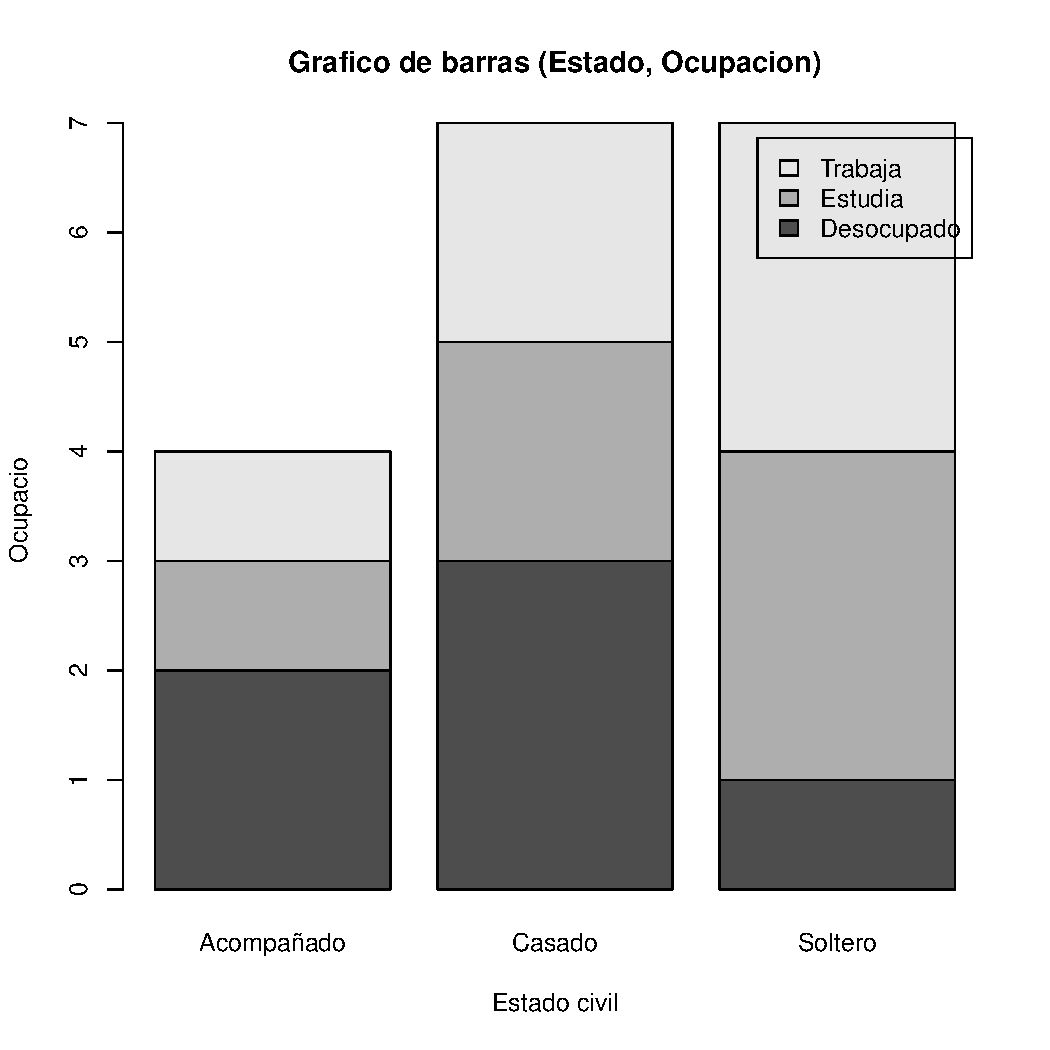
\includegraphics[width=\maxwidth]{figure/unnamed-chunk-1-1} 
\begin{kframe}\begin{alltt}
\hlstd{sw} \hlkwb{<-} \hlkwd{shapiro.test}\hlstd{(IMC_Control)}
\hlstd{sw}
\end{alltt}
\begin{verbatim}
## 
## 	Shapiro-Wilk normality test
## 
## data:  IMC_Control
## W = 0.95321, p-value = 0.4776
\end{verbatim}
\begin{alltt}
\hlstd{ks} \hlkwb{<-} \hlkwd{ks.test}\hlstd{(IMC_Control,}\hlstr{"pnorm"}\hlstd{,}\hlkwc{mean}\hlstd{=}\hlkwd{mean}\hlstd{(IMC_Control),}\hlkwc{sd}\hlstd{=}\hlkwd{sd}\hlstd{(IMC_Control))}
\hlstd{ks}
\end{alltt}
\begin{verbatim}
## 
## 	One-sample Kolmogorov-Smirnov test
## 
## data:  IMC_Control
## D = 0.11172, p-value = 0.9595
## alternative hypothesis: two-sided
\end{verbatim}
\begin{alltt}
\hlcom{#Luego se digitan los datos para pacientes y se ejecutan las mismas instrucciones}
\hlstd{IMC_Pacientes} \hlkwb{<-} \hlkwd{c}\hlstd{(}\hlnum{25.6}\hlstd{,} \hlnum{22.7}\hlstd{,} \hlnum{25.9}\hlstd{,} \hlnum{24.3}\hlstd{,} \hlnum{25.2}\hlstd{,} \hlnum{29.6}\hlstd{,} \hlnum{21.3}\hlstd{,} \hlnum{25.5}\hlstd{,} \hlnum{27.4}\hlstd{,}
                   \hlnum{22.3}\hlstd{,} \hlnum{24.4}\hlstd{,} \hlnum{23.7}\hlstd{,} \hlnum{20.6}\hlstd{,} \hlnum{22.8}\hlstd{)}

\hlkwd{par}\hlstd{(}\hlkwc{mfrow}\hlstd{=}\hlkwd{c}\hlstd{(}\hlnum{1}\hlstd{,}\hlnum{2}\hlstd{))}
\hlkwd{hist}\hlstd{(IMC_Pacientes,}\hlkwc{main}\hlstd{=}\hlstr{"A"}\hlstd{,}\hlkwc{xlab}\hlstd{=}\hlstr{"IMC (kg/m2)"}\hlstd{,}\hlkwc{ylab}\hlstd{=}\hlstr{"Frecuencia"}\hlstd{)}
\hlkwd{boxplot}\hlstd{(IMC_Pacientes,}\hlkwc{main}\hlstd{=}\hlstr{"B"}\hlstd{,} \hlkwc{lab}\hlstd{=}\hlstr{"IMC (kg/m2)"}\hlstd{,}\hlkwc{ylim}\hlstd{=}\hlkwd{c}\hlstd{(}\hlnum{20}\hlstd{,}\hlnum{30}\hlstd{))}
\end{alltt}
\end{kframe}
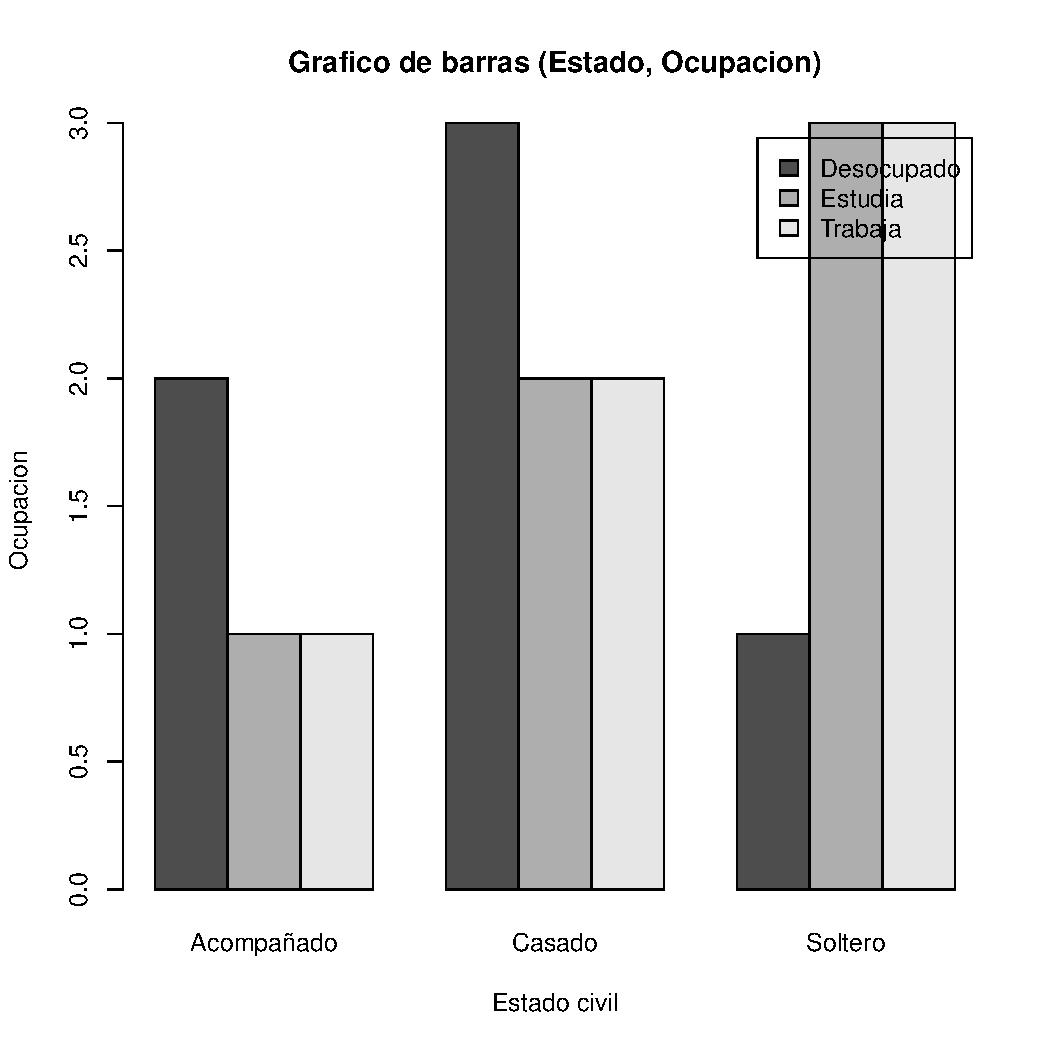
\includegraphics[width=\maxwidth]{figure/unnamed-chunk-1-2} 
\begin{kframe}\begin{alltt}
\hlstd{sw} \hlkwb{<-} \hlkwd{shapiro.test}\hlstd{(IMC_Pacientes)}
\hlstd{sw}
\end{alltt}
\begin{verbatim}
## 
## 	Shapiro-Wilk normality test
## 
## data:  IMC_Pacientes
## W = 0.97437, p-value = 0.929
\end{verbatim}
\begin{alltt}
\hlstd{ks} \hlkwb{<-} \hlkwd{ks.test}\hlstd{(IMC_Pacientes,}\hlstr{"pnorm"}\hlstd{,}\hlkwc{mean}\hlstd{=}\hlkwd{mean}\hlstd{(IMC_Pacientes),}\hlkwc{sd}\hlstd{=}\hlkwd{sd}\hlstd{(IMC_Pacientes))}
\hlstd{ks}
\end{alltt}
\begin{verbatim}
## 
## 	One-sample Kolmogorov-Smirnov test
## 
## data:  IMC_Pacientes
## D = 0.12172, p-value = 0.9695
## alternative hypothesis: two-sided
\end{verbatim}
\end{kframe}
\end{knitrout}



\end{document}
